\documentclass[10pt,letterpaper]{article}
\usepackage[top=0.85in,left=2.75in,footskip=0.75in]{geometry}

% amsmath and amssymb packages, useful for mathematical formulas and symbols
\usepackage{amsmath,amssymb}

\usepackage{graphicx}

% Use adjustwidth environment to exceed column width (see example table in text)
\usepackage{changepage}

% Use Unicode characters when possible
\usepackage{inputenc}

% textcomp package and marvosym package for additional characters
\usepackage{textcomp,marvosym}

% cite package, to clean up citations in the main text. Do not remove.
\usepackage{cite}

% Use nameref to cite supporting information files (see Supporting Information section for more info)
\usepackage{nameref,hyperref}

% line numbers
\usepackage[right]{lineno}

% ligatures disabled
\usepackage{microtype}
\DisableLigatures[f]{encoding = *, family = * }

% color can be used to apply background shading to table cells only
\usepackage[table]{xcolor}

% array package and thick rules for tables
\usepackage{array}

\usepackage{algorithm}
\usepackage{algpseudocode}

\usepackage{float}
\usepackage{timestamp}

%% Include all macros below

\newcommand{\lorem}{{\bf LOREM}}
\newcommand{\ipsum}{{\bf IPSUM}}

%% END MACROS SECTION
\newcommand{\R}{\mathbb{R}}

\begin{document}
\vspace*{0.2in}

% Title must be 250 characters or less.
\begin{flushleft}
{\Large
\textbf\newline{A Monte Carlo method to estimate cell population heterogeneity}
}
\newline
\\
Ben Lambert\textsuperscript{1,2}*,
David J. Gavaghan\textsuperscript{3},
Simon Tavener\textsuperscript{4}.
\\
\bigskip
\textbf{1} Department of Zoology, University of Oxford, Oxford, Oxfordshire, U.K.
\\
\textbf{2} MRC Centre for Outbreak Analysis and Modelling, Infectious Disease Epidemiology, Imperial College London, London W2 1PG, UK.
\\
\textbf{3} Department of Computer Science, University of Oxford, Oxford, U.K.
\\
\textbf{4} Department of Statistics, Colorado State University, Fort Collins, Colorado, U.S.A.
\\
\bigskip

% Use the asterisk to denote corresponding authorship and provide email address in note below.
*ben.c.lambert@gmail.com.

\end{flushleft}

\hfill Revision date \& time: \timestamp
\bigskip


% Please keep the abstract below 300 words
%%%%%%%%%%%%%%%%%%%%%%%%%%%%%%%%%%%%%%%%%%%%%%%%%%%%%%%%%%%%%%%%%%%%%%%%%%%%%%%%%%%%%%%%%%%%%%%%%%%%%%%%%%%%%%%%%%%%%%%%                                                                                                                  %                                                                                                                      %
%       ABSTRACT                                                                                                       %
%                                                                                                                      %
%%%%%%%%%%%%%%%%%%%%%%%%%%%%%%%%%%%%%%%%%%%%%%%%%%%%%%%%%%%%%%%%%%%%%%%%%%%%%%%%%%%%%%%%%%%%%%%%%%%%%%%%%%%%%%%%%%%%%%%%

% The Abstract of the paper should be succinct; it must not exceed 300 words. Authors should mention the techniques used without going into methodological detail and should summarize the most important results.

% While the Abstract is conceptually divided into three sections (Background, Methodology/Principal Findings, and Conclusions/Significance), do not apply these distinct headings to the Abstract within the article file.

% Do not include any citations. Avoid specialist abbreviations.
\newpage
\section{Abstract}
Variation is characteristic of all living systems. Laboratory techniques, such as flow cytometry, have been used to probe individual cells in a population and, after decades of experimentation, it is clear that even seemingly identical cells exhibit differences. To understand whether this variation is biologically meaningful, it is essential to discern its source. Mathematical models of biological systems provide a tool that can be used to investigate the source of cell-to-cell variation. From mathematical analysis and simulation of these models, hypotheses leading to different system behaviours can be posed. Parameter inference provides a means to test which of these hypotheses are most compatible with experimental data. Data from laboratory experiments often takes the form of ``snapshots" representing distributions of cellular properties at different points in times, rather than individual cell trajectories. This data is not straightforward to fit using hierarchical Bayesian methods since it requires inferring the identities of the groups to which individual cells belong. Further, such grouping may be biologically dubious since variation may be better represented by a spectrum of characteristics rather than categorical bins. Here, we introduce a computational sampling method we call ``Contour Monte Carlo" for estimating mathematical model parameters from snapshot distributions which is straightforward to implement and does not require explicitly assigning cells to categories. Our method is most applicable to systems where the dominant source of variation is cell-to-cell heterogeneity in cellular processes rather than experimental measurement error which, due to the increasingly finescale resolution of laboratory techniques, may be the case for a wide class of systems. In this paper, we illustrate the use of our method to estimate cellular variation for three systems of biological interest and provide code in the form of a Julia notebook which allows others to apply this approach to their problem.


\section{Introduction}
Variation rather than homogeneity is the rule rather than exception in biology. Indeed, without variation, biology as a discipline would not exist, since as evolutionary biologist JBS Haldane wrote, variation is the ``raw material" of evolution. The Red Queen Hypothesis asserts that organisms must continually evolve in order to survive when pitted against other - also evolving - organisms \cite{ridley1994red}. A corollary of this hypothesis is that multicellular organisms may evolve cellular phenotypic heterogeneity to allow for faster adaptation to changing environments, which may explain the observed variation in a range of biological systems \cite{fraser2009chance}. Whilst cell population variation can confer evolutionary advantages, it may be costly to particular applications. In biotechnological processes, heterogeneity in cellular function can lead to reduced yields of biochemical products \cite{delvigne2014metabolic}. In developing therapeutics, variation is also often undesirable since treatments typically aim to steer modal cellular properties and may fail to influence key subpopulations. For example, cellular heterogeneity likely allows cancerous tumours to persist \cite{gatenby2007cellular} and evolve resistance to chemotherapies over time \cite{altrock2015mathematics}. Identifying sources of variation in populations of cells is thus important to determine whether this has functional significance for a wide range of applications.

Mathematical models are essential tools for making sense of cellular systems, whose emergent properties are the result of complex interactions between various actors. Perhaps the simplest flavour of mathematical model used in biological systems are ordinary differential equations (ODEs) that lump individual actors into partitions according to structure or function, and seek to model the mean behaviour of each partition. Data from population-averaged experimental assays can be a powerful resource to understand whether such models faithfully reproduce system behaviours and can allow for quantification of the interactions of various cellular components of complex metabolic, signalling and transciptional networks. The worth of such models however is determined by whether averages mask differences in behaviour of individual cells that result in functional consequences \cite{altschuler2010cellular}. For example, differences in cellular protein abundances due to biochemical ``noise" may not be meaningful biologically \cite{elowitz2002stochastic} and so mean cell behaviour suffices as a description of the system. Such noise may have functional consequences however. For example, a recent study demonstrated that subpopulations of clonally derived hematopoietic progenitor cells with low or high expression of a particular stem cell marker produced different blood lineages \cite{chang2008transcriptome}. 

To accommodate cell population heterogeneity in mathematical models, a variety of modelling choices are available, each posing different challenges for parameter inference, and are described in a recent review \cite{waldherr2018estimation}. These include modelling biochemical processes stochastically, resulting in the properties of an ensemble of cells being represented by a probability distribution which evolves according to a chemical master equation (see \cite{erban2007practical} for a tutorial on stochastic reaction-diffusion processes; RDEs). Alternatively, a population balance equation (PBE) can be used to dictate the evolution of the ``number density" of cells of differing cell types, whose properties are represented as points in $\mathbb{R}^n$ which, in turn, affect their function, including their rate of death and cell division (see \cite{ramkrishna2014population} for an introduction to PBEs). In a PBE approach, variation in measured quantities results primarily due to differing functional properties of heterogeneous cell types and variation in the initial densities of these variants. 

The approach we follow here is similar to that of \cite{dixit2018maximum}, wherein dynamic cellular variation is generated by describing the evolution of each cell's state using an ODE, but with individual cell differences in the rate parameters of the process. For sake of reference throughout this paper, we deem these models as ``heterogenous ODEs (HODEs)". In HODEs, the aim of inference is to estimate the distributions of parameter values across cells consistent with observed distributions of measurements at various timepoints. A benefit of using HODEs to model cell heterogeneity is that these models are computationally straightforward to simulate and, arguably, simpler to parameterise than PBEs. In these models the predominant source of variation is due to differences in cellular processes between cells not due to inherent stochasticity in biochemical reactions within cells, as in stochastic RDEs.

The difficulty of performing inference on HODEs is partly due to experimental hurdles in generating data of sufficient quality to allow identification. Unlike models which represent a population by a single scalar ODE, HODEs require individual cell data for estimation. A widely-used method for generating data for individual cells is flow cytometry, where a large number of cells are streamed individually through a laser beam and, for example, abundance measurements made of proteins labelled with fluorescent markers \cite{telford2012flow}. Alternatively, experimental techniques such as Western blotting and cytometric fluorescence microscopy can generate single cell measurements \cite{hughes2014single,hasenauer2011identification}. A property of these experimental methods is that they are destructive, meaning that individual cells are sacrificed as part of the measurement process. This means that the measurements of cell properties conducted at a certain point in time represent what are termed ``snapshots" of the underlying population \cite{hasenauer2011identification}. These snapshots are often described by histograms \cite{dixit2018maximum} or density functions \cite{waldherr2018estimation} fit to the underlying data at different points in time (Fig. X). Since HODEs represent the underlying state of individual cells as evolving continuously through time, corresponding data showing individual cell trajectories constitutes a richer data resource.


Mention Loos paper re: hierarchical.



Figure where we show the workflow for inverse-sensitivity analysis, including comparing output data to targets.

Figure where we explain why Bayesian hierarchical modelling is difficult for snapshot data.





\linenumbers


In Bayesian parameter estimation, the aim is to estimate probability distributions over parameter values consistent with given output data series (Fig ). In inverse sensitivity analysis, the aim is similar, except that parameter distributions resulting in output distributions, not data, are sought (Fig ). In Bayesian models of dynamic systems, it is common practice to assume a state-space framework to explain variation in data. In non-hierarchical state-space models, the data sample is assumed to result from a single ``true" state of nature coupled with a noisy measurement process. This measurement process induces variation in the sample at a given time even if the state evolves deterministically. In inverse sensitivity analysis of deterministic models, the variation in outputs represented by probability distributions is supposed to be the result of stochasticity in parameter values, across each of many replicates of a process. That is, the randomness is due to variation in the underlying state not due to an imperfect measurement process. Which of these sources of variation predominates depends on circumstance. Suppose we use a deterministic SIR model to describe the prevalence of an infectious disease in a small region. In this case, there are no replicates of the process and the number of observed cases will be a noisy measure of the true (unobserved) case counts due to the imperfect sensitivity and specificity of diagnostic approaches taken. Instead imagine that we accurately record the level of a signalling protein in individual cells over time using flow cytometry, resulting in snapshot distributions of protein levels at different points in time. Here, the dominant source of stochasticity may be cell-to-cell variation in the underlying processes that produce the protein. Additionally, since individual cells cannot be matched up with themselves at different points in time, the data provided is in the form of summary distributions rather than individual trajectories of cells over time, meaning hierarchical Bayesian models are less well suited. In this context, inverse sensitivity analysis is applicable and allows estimation of the underlying variation in the process parameters across cells.

Due to the differing aims and assumed sources of stochasticity, the posterior parameter distributions that result from non-hierarchical Bayesian inference or inverse sensitivity have different interpretations. For these Bayesian models, the posterior distributions represent our underlying epidemic uncertainty over a single set of true parameter values. For inverse sensitivity analyses, they indicate the degree of ontological (that is, actually occurring) variation in parameter values across units of measurement. Hierarchical Bayesian models allow for variation in the parameters that determine the evolution of the state across measurement groups and uncertainty due to measurement error. Accordingly, the posteriors for the so-called ``hyperparameters" of these models indicate variation due to cell-to-cell variability, whereas posteriors for group-level parameters indicate our epistemic uncertainty in these estimates. Thus, it is possible to discern a spectrum of problem types: at one end there are non-hierarchical Bayesian models, where the posteriors indicate our epistemic uncertainty in parameter values; at the other end, inverse sensitivity problems sit, where the posteriors indicate actual unit-to-unit variation in parameter values; somewhere in the middle are Bayesian hierarchical models, which incorporate both types of variation. A subtle difference however with inverse sensitivity models however is that their starting point is output distributions rather than output data used in the Bayesian models. 

\begin{figure}[H]
	\centerline{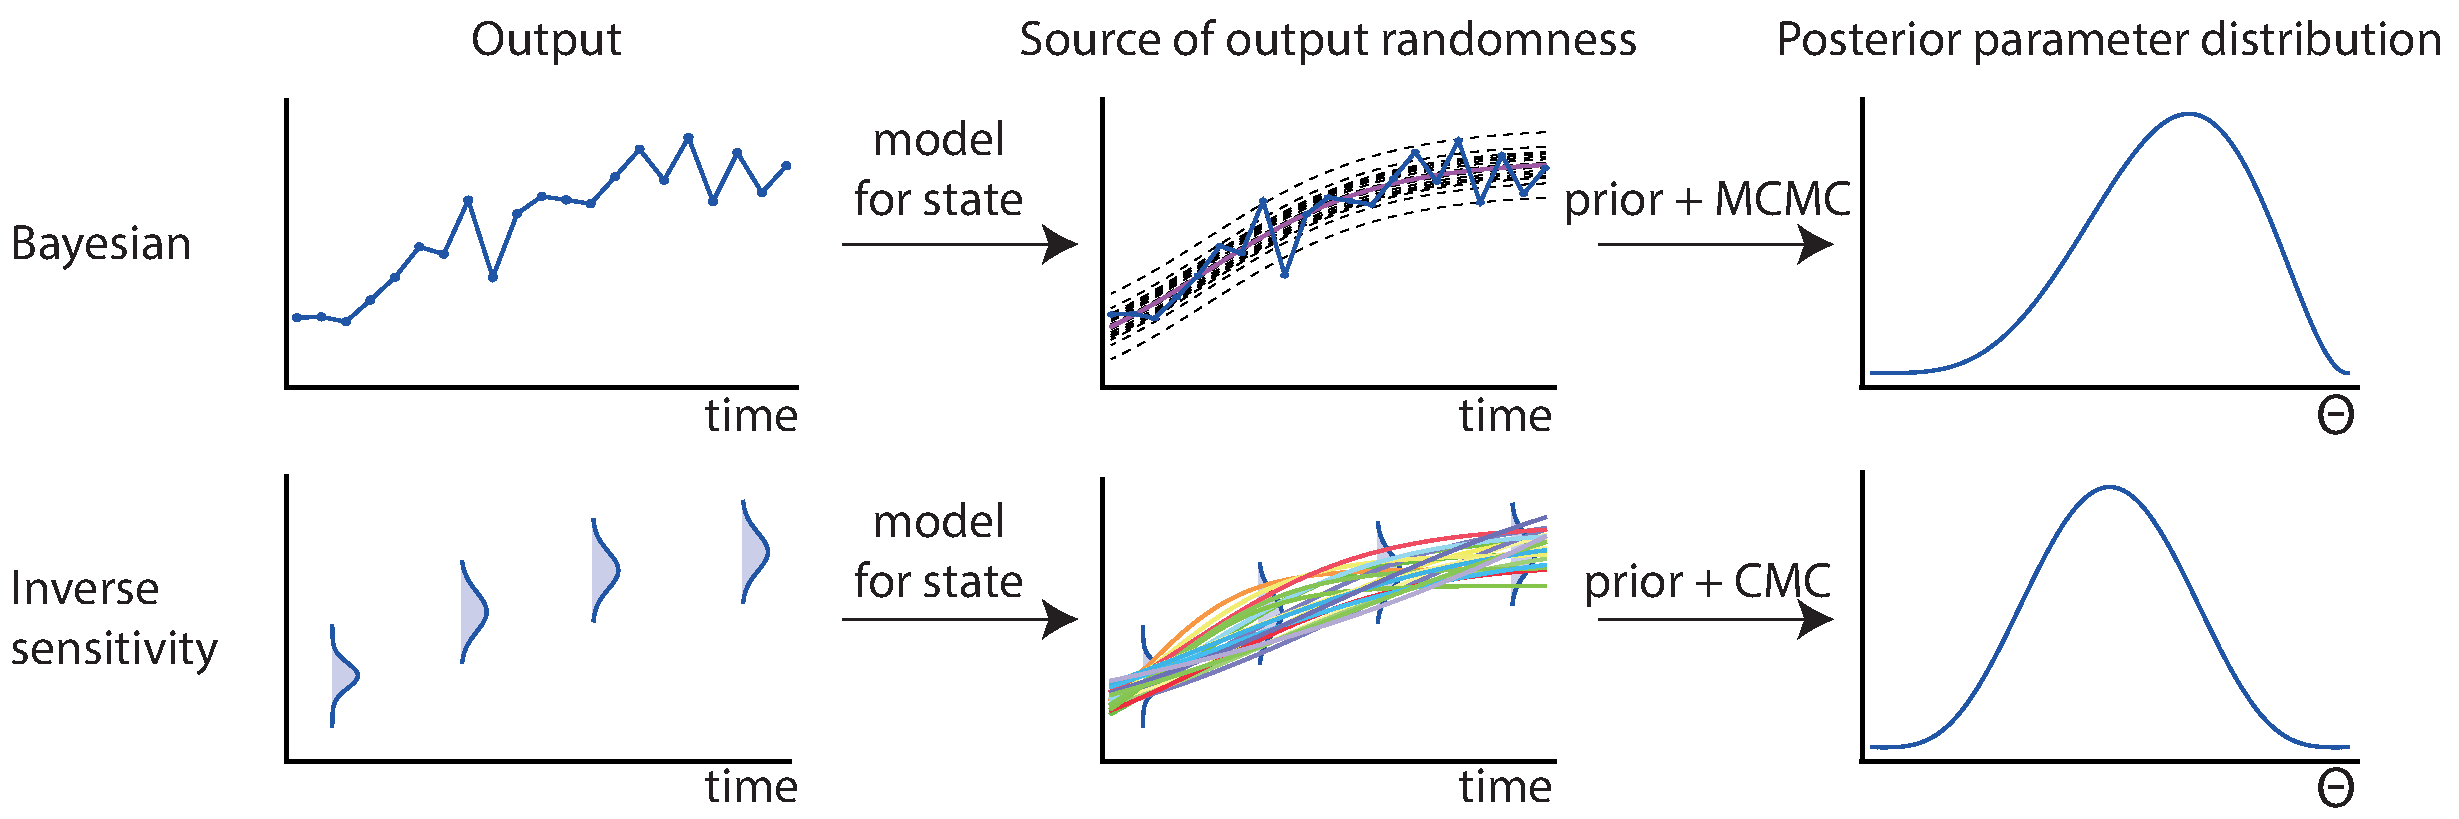
\includegraphics[width=1.25\textwidth]{../figures/comparing_bayes_sensitivity.pdf}}
	\caption{\textbf{The difference between non-hierarchical Bayesian inference (top row) and inverse sensitivity analysis (bottom row).} The left hand column indicates the output information which is used to perform parameter inference in each case. The middle column indicates the source of output variation: for Bayesian state-space models this is often the measurement error process whereas for deterministic dynamic models this is stochasticity in the underlying parameter values. The right hand column shows example posterior distributions that would result from each analysis.}
	\label{fig:difference_between_bayes_invsensitivity}
\end{figure}

For a large class of models of practical interest in biology, including ordinary differential equations (ODEs) and partial differential equations (PDEs), analytic methods for inverse sensitivity analysis  are unavailable. Further it is common for the dimension of the inputs to exceed that of the outputs. For deterministic systems, this means that there exist non-singular sets of inputs that can yield a given output and that any feasible output distribution may be caused by any member of a collection of possible input distributions. In Bayesian inference of stochastic systems, prior distributions are specified for parameters of the likelihood ensuring a unique input distribution for a given set of output data. For deterministic models, however, there is no uncertainty in the input-to-output map, meaning standard Bayesian techniques cannot be used without introducing an artificial error distribution. Here we describe a conceptual framework to understand the inversion of deterministic systems. We then describe a novel Markov Chain Monte Carlo method we call ``Contour Monte Carlo'' and use this approach to invert a number of systems, including the logistic growth equation, the Michaelis-Menten equation, and an SIR model of disease transmission. In contrast to methods that use a grid to discretize the parameter domain to determine a numerical output-to-input map \cite{butler2014measure}, our method uses stochastic sampling to instead approximate the multiplicity of a given output value; that is, the number of inputs that map to that value. By using random sampling, the computational complexity of our approach does not grow with parameter dimensions, meaning that it can be applied to large model systems. We also argue that the simplicity of our approach means it is amenable to a large class of problems of practical significance.


\bigskip
\noindent\underline{Outline of the paper}: In \S \ref{sec:methods}, we present the basic CMC algorithm assuming uniform priors in \S \ref{sec:uniform_priors}, and extend this approach to general prior distributions in \S \ref{sec:general_priors}. In \S \ref{sec:illustrativeExamples}, we examine several algebraic examples to illustrate how the CMC algorithm works in detail. CMC is then used to invert a range of examples drawn from mathematical biology in \S \ref{sec:results} before a discussion in \S \ref{sec:discussion}.



\section{Discussion}
\label{sec:discussion}

Natural selection has dictated that organisms have often evolved redundancies for systems essential for life. By building mathematical models we aim to mimic these systems, meaning that these models should embody similar redundancies as their biological counterparts. Assessing the sensitivity of key characteristics of model outputs to perturbations in input parameters provides insight into the sensitivity of the system to each of its constituent elements. These so-called sensitivity analyses of mathematical models allow us to probe the biological system even when biological experiments are infeasible. Inverse sensitivity analysis inverts this process and instead of determining how model outputs vary in response to changes to the input parameter values, estimates a distribution over inputs which achieves a given distribution over outputs.

In this paper, we introduce an approach to inverse sensitivity analysis which can be applied to systems with many input parameters, mitigating the curse of dimensionality that limits the scope of  methods which rely on grid-based approaches to build an explicit output-to-input map \cite{butler2014measure}. We have demonstrated that our algorithms can perform inverse sensitivity analysis on mathematical models of biological systems across a range of complexities, including the logistic growth model (2 inputs \& 1 output target), Michaelis-Menten kinetics (3 inputs \& 2 output targets), and the SIR model with uncertain initial population sizes (9 inputs \& 3 output targets). As well as detailing our algorithms, we provide a probabilistic framework for understanding inverse sensitivity analysis, in which ``prior'' probability distributions are set on the inputs. These prior beliefs over input values are consistent with a ``posterior'' input distribution which, when transformed through the input-to-output map, results in a ``target'' output distribution. To sample from these posterior input distributions, we introduce a two-step sampling algorithm. In the first of these steps, input parameters are independently sampled from their prior distributions and, by fitting a kernel density estimator to the output values, this provides an approximate Jacobian transform (which we interchangeably term a ``contour volume distribution''), which is used in the second step involving Markov chain Monte Carlo. A similar algorithm for inverse sensitivity analysis has recently been derived from a measure theoretic perspective by \cite{BJW-17}. These authors also investigate stability of the posterior distribution with respect to the observed output distribution, the assumed prior distribution and the approximation of the contours of the forward map. We believe that the different path we take to the shared goal offers complementary insight into the algorithm's mechanism and provides an intuitive way to understand inverse sensitivity analysis, more generally.

There are several subtleties in the first steps of the processes described in Algorithms \ref{alg:constrained} and \ref{alg:unconstrained}) which must be understood in order to ensure a valid input distribution is obtained. Indeed, these intricacies complicated our own efforts in testing the algorithms. Provided the output is well-behaved over the space of possible input values, a univariate output distribution can be approximated given a relatively modest number of samples from the input priors using standard kernel density estimation (KDE). Here, for the univariate output target distributions we found that KDE with a Gaussian kernel using default bandwidths from each software package used (Matlab, Mathematica and R \cite{MATLAB:2016,mathematica,RLanguage}) was able to represent the output distribution with sufficient fidelity to ensure the input posterior recaptured the output target. The number of input samples necessary to ensure convergence to the true posterior input distribution, however, depends on the exact output distribution being targeted. If the bulk of probability mass for the target output distribution lies at a location in output space where the contour volume is rapidly varying, then the input distribution obtained will be sensitive to errors in kernel density estimates of the contour volume distribution, and many samples will be required. Similarly, if a region of low contour volume is targeted, then kernel density estimates with few samples will be relatively noisy and more samples will be necessary. Here we have assumed numerical errors in solving the map are negligible and independent of the parameters. Neither assumption is likely to be true for sophisticated partial differential equation models and the interaction between numerical and sampling errors is the subject of ongoing analysis. KDE introduces a further source of error, which must be carefully managed to ensure reasonable results are obtained.

Our algorithms avoid the curse of dimensionality of the input space which plagues grid-based approaches to inverse sensitivity analysis. The necessity of having to fit a probability distribution to the output samples resultant from sampling the prior input distributions means that, at present, our approach is limited to problems with relatively few outputs. In \S \ref{sec:SIR}, the output target was a three-dimensional distribution, and we expended considerable effort finding a KDE method that adequately approximated the three-dimensional contour volume distribution. We ultimately found that the most effective approach was obtained by using the ``kde'' function within the ``ks'' R package \cite{duong2018package,RLanguage}, which uses the data to estimate unconstrained bandwidth matrices, which are then used to fit kernel density estimates to data with up to six dimensions. Density estimation, however, is currently an active area of research and software packages exist implementing many different variants of KDE (see \cite{deng2011density} for a review of the R packages already available in 2011). Vine copulas have recently been suggested as an approach which avoids the curse of dimensionality in density estimation \cite{nagler2016evading}. If this promise is realised, then our algorithm will be applicable to output target distributions of higher dimensions.

Mathematical models have proved indispensable tools for elucidating understanding of biological systems, which are frequently not amenable to direct experimentation. Biological systems are often robust to perturbations to particular constituent processes, and we can use mathematical models to explore these sensitivities. Inverse sensitivity analyses are a relatively recent addition to a modeller's toolbox, which allows one to determine an input distribution - consistent with prior beliefs - that can generate a given distribution of outputs. Here we introduce a Monte Carlo method which extends the range of models for which inverse sensitivity analysis can be performed, and illustrate its utility for several problems of interest to computational biology. It is our hope that, by publishing this method, others are encouraged to undertake inverse sensitivity analysis, which we have found is insightful for building and analysing mathematical models.

\section{Author contributions}
BL, DJG and SJT conceived the study. BL and SJT carried out the analysis. All authors helped to write and edit the manuscript.


\nolinenumbers

\bibliographystyle{unsrt}
\bibliography{Bayes}

\section*{Supporting information captions}
\begin{itemize}
  \item S1--Michaelis-Menten kinetics
  \item S2--SIR model
  \item S3--A nonlinear map
\end{itemize}

\end{document}

